% Created by tikzDevice version 0.12.6 on 2024-02-19 10:07:45
% !TEX encoding = UTF-8 Unicode
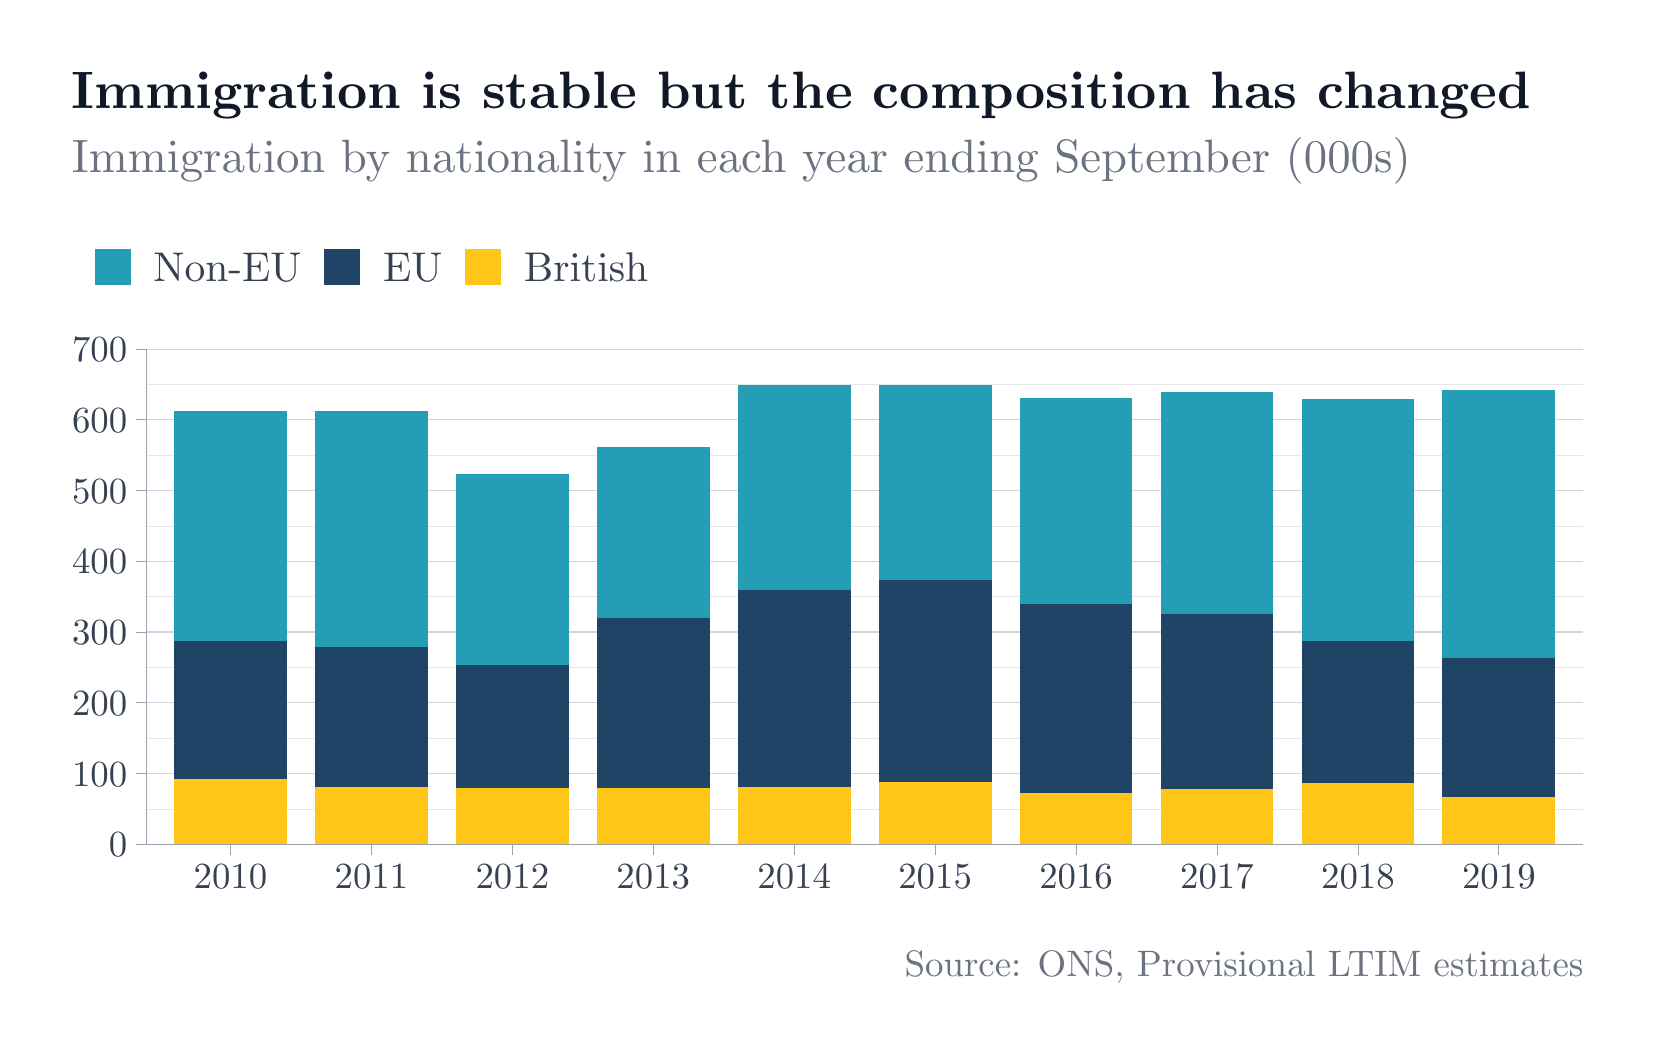
\begin{tikzpicture}[x=1pt,y=1pt]
\definecolor{fillColor}{RGB}{255,255,255}
\path[use as bounding box,fill=fillColor] (0,0) rectangle (578.16,361.35);
\begin{scope}
\path[clip] (  0.00,  0.00) rectangle (578.16,361.35);
\definecolor{drawColor}{RGB}{255,255,255}

\path[draw=drawColor,line width= 0.8pt,line join=round,line cap=round,fill=fillColor] ( -0.00,  0.00) rectangle (578.16,361.35);
\end{scope}
\begin{scope}
\path[clip] ( 42.74, 66.29) rectangle (562.16,245.20);
\definecolor{drawColor}{RGB}{255,255,255}
\definecolor{fillColor}{RGB}{255,255,255}

\path[draw=drawColor,line width= 0.8pt,line join=round,line cap=round,fill=fillColor] ( 42.74, 66.29) rectangle (562.16,245.20);
\definecolor{drawColor}{RGB}{229,231,235}

\path[draw=drawColor,line width= 0.2pt,line join=round] ( 42.74, 79.07) --
	(562.16, 79.07);

\path[draw=drawColor,line width= 0.2pt,line join=round] ( 42.74,104.63) --
	(562.16,104.63);

\path[draw=drawColor,line width= 0.2pt,line join=round] ( 42.74,130.19) --
	(562.16,130.19);

\path[draw=drawColor,line width= 0.2pt,line join=round] ( 42.74,155.75) --
	(562.16,155.75);

\path[draw=drawColor,line width= 0.2pt,line join=round] ( 42.74,181.31) --
	(562.16,181.31);

\path[draw=drawColor,line width= 0.2pt,line join=round] ( 42.74,206.86) --
	(562.16,206.86);

\path[draw=drawColor,line width= 0.2pt,line join=round] ( 42.74,232.42) --
	(562.16,232.42);
\definecolor{drawColor}{RGB}{209,213,219}

\path[draw=drawColor,line width= 0.4pt,line join=round] ( 42.74, 66.29) --
	(562.16, 66.29);

\path[draw=drawColor,line width= 0.4pt,line join=round] ( 42.74, 91.85) --
	(562.16, 91.85);

\path[draw=drawColor,line width= 0.4pt,line join=round] ( 42.74,117.41) --
	(562.16,117.41);

\path[draw=drawColor,line width= 0.4pt,line join=round] ( 42.74,142.97) --
	(562.16,142.97);

\path[draw=drawColor,line width= 0.4pt,line join=round] ( 42.74,168.53) --
	(562.16,168.53);

\path[draw=drawColor,line width= 0.4pt,line join=round] ( 42.74,194.08) --
	(562.16,194.08);

\path[draw=drawColor,line width= 0.4pt,line join=round] ( 42.74,219.64) --
	(562.16,219.64);

\path[draw=drawColor,line width= 0.4pt,line join=round] ( 42.74,245.20) --
	(562.16,245.20);
\definecolor{fillColor}{RGB}{255,197,23}

\path[fill=fillColor] ( 52.92, 66.29) rectangle ( 93.66, 89.81);

\path[fill=fillColor] (103.85, 66.29) rectangle (144.59, 87.00);

\path[fill=fillColor] (154.77, 66.29) rectangle (195.51, 86.48);

\path[fill=fillColor] (205.70, 66.29) rectangle (246.43, 86.48);

\path[fill=fillColor] (256.62, 66.29) rectangle (297.36, 87.00);

\path[fill=fillColor] (307.54, 66.29) rectangle (348.28, 88.78);

\path[fill=fillColor] (358.47, 66.29) rectangle (399.20, 84.70);

\path[fill=fillColor] (409.39, 66.29) rectangle (450.13, 86.23);

\path[fill=fillColor] (460.31, 66.29) rectangle (501.05, 88.27);

\path[fill=fillColor] (511.24, 66.29) rectangle (551.98, 83.42);
\definecolor{fillColor}{RGB}{32,68,102}

\path[fill=fillColor] ( 52.92, 89.81) rectangle ( 93.66,139.65);

\path[fill=fillColor] (103.85, 87.00) rectangle (144.59,137.60);

\path[fill=fillColor] (154.77, 86.48) rectangle (195.51,131.21);

\path[fill=fillColor] (205.70, 86.48) rectangle (246.43,148.08);

\path[fill=fillColor] (256.62, 87.00) rectangle (297.36,158.30);

\path[fill=fillColor] (307.54, 88.78) rectangle (348.28,161.88);

\path[fill=fillColor] (358.47, 84.70) rectangle (399.20,152.94);

\path[fill=fillColor] (409.39, 86.23) rectangle (450.13,149.61);

\path[fill=fillColor] (460.31, 88.27) rectangle (501.05,139.90);

\path[fill=fillColor] (511.24, 83.42) rectangle (551.98,133.51);
\definecolor{fillColor}{RGB}{36,157,181}

\path[fill=fillColor] ( 52.92,139.65) rectangle ( 93.66,222.97);

\path[fill=fillColor] (103.85,137.60) rectangle (144.59,222.97);

\path[fill=fillColor] (154.77,131.21) rectangle (195.51,199.96);

\path[fill=fillColor] (205.70,148.08) rectangle (246.43,209.93);

\path[fill=fillColor] (256.62,158.30) rectangle (297.36,232.17);

\path[fill=fillColor] (307.54,161.88) rectangle (348.28,232.17);

\path[fill=fillColor] (358.47,152.94) rectangle (399.20,227.57);

\path[fill=fillColor] (409.39,149.61) rectangle (450.13,229.87);

\path[fill=fillColor] (460.31,139.90) rectangle (501.05,227.31);

\path[fill=fillColor] (511.24,133.51) rectangle (551.98,230.38);

\path[] ( 42.74, 66.29) rectangle (562.16,245.20);
\end{scope}
\begin{scope}
\path[clip] (  0.00,  0.00) rectangle (578.16,361.35);
\definecolor{drawColor}{RGB}{156,163,175}

\path[draw=drawColor,line width= 0.3pt,line join=round] ( 42.74, 66.29) --
	( 42.74,245.20);
\end{scope}
\begin{scope}
\path[clip] (  0.00,  0.00) rectangle (578.16,361.35);
\definecolor{drawColor}{RGB}{55,65,81}

\node[text=drawColor,anchor=base east,inner sep=0pt, outer sep=0pt, scale=  1.33] at ( 35.99, 61.70) {0};

\node[text=drawColor,anchor=base east,inner sep=0pt, outer sep=0pt, scale=  1.33] at ( 35.99, 87.26) {100};

\node[text=drawColor,anchor=base east,inner sep=0pt, outer sep=0pt, scale=  1.33] at ( 35.99,112.82) {200};

\node[text=drawColor,anchor=base east,inner sep=0pt, outer sep=0pt, scale=  1.33] at ( 35.99,138.38) {300};

\node[text=drawColor,anchor=base east,inner sep=0pt, outer sep=0pt, scale=  1.33] at ( 35.99,163.94) {400};

\node[text=drawColor,anchor=base east,inner sep=0pt, outer sep=0pt, scale=  1.33] at ( 35.99,189.49) {500};

\node[text=drawColor,anchor=base east,inner sep=0pt, outer sep=0pt, scale=  1.33] at ( 35.99,215.05) {600};

\node[text=drawColor,anchor=base east,inner sep=0pt, outer sep=0pt, scale=  1.33] at ( 35.99,240.61) {700};
\end{scope}
\begin{scope}
\path[clip] (  0.00,  0.00) rectangle (578.16,361.35);
\definecolor{drawColor}{RGB}{156,163,175}

\path[draw=drawColor,line width= 0.3pt,line join=round] ( 38.99, 66.29) --
	( 42.74, 66.29);

\path[draw=drawColor,line width= 0.3pt,line join=round] ( 38.99, 91.85) --
	( 42.74, 91.85);

\path[draw=drawColor,line width= 0.3pt,line join=round] ( 38.99,117.41) --
	( 42.74,117.41);

\path[draw=drawColor,line width= 0.3pt,line join=round] ( 38.99,142.97) --
	( 42.74,142.97);

\path[draw=drawColor,line width= 0.3pt,line join=round] ( 38.99,168.53) --
	( 42.74,168.53);

\path[draw=drawColor,line width= 0.3pt,line join=round] ( 38.99,194.08) --
	( 42.74,194.08);

\path[draw=drawColor,line width= 0.3pt,line join=round] ( 38.99,219.64) --
	( 42.74,219.64);

\path[draw=drawColor,line width= 0.3pt,line join=round] ( 38.99,245.20) --
	( 42.74,245.20);
\end{scope}
\begin{scope}
\path[clip] (  0.00,  0.00) rectangle (578.16,361.35);
\definecolor{drawColor}{RGB}{156,163,175}

\path[draw=drawColor,line width= 0.3pt,line join=round] ( 42.74, 66.29) --
	(562.16, 66.29);
\end{scope}
\begin{scope}
\path[clip] (  0.00,  0.00) rectangle (578.16,361.35);
\definecolor{drawColor}{RGB}{156,163,175}

\path[draw=drawColor,line width= 0.3pt,line join=round] ( 73.29, 62.54) --
	( 73.29, 66.29);

\path[draw=drawColor,line width= 0.3pt,line join=round] (124.22, 62.54) --
	(124.22, 66.29);

\path[draw=drawColor,line width= 0.3pt,line join=round] (175.14, 62.54) --
	(175.14, 66.29);

\path[draw=drawColor,line width= 0.3pt,line join=round] (226.06, 62.54) --
	(226.06, 66.29);

\path[draw=drawColor,line width= 0.3pt,line join=round] (276.99, 62.54) --
	(276.99, 66.29);

\path[draw=drawColor,line width= 0.3pt,line join=round] (327.91, 62.54) --
	(327.91, 66.29);

\path[draw=drawColor,line width= 0.3pt,line join=round] (378.84, 62.54) --
	(378.84, 66.29);

\path[draw=drawColor,line width= 0.3pt,line join=round] (429.76, 62.54) --
	(429.76, 66.29);

\path[draw=drawColor,line width= 0.3pt,line join=round] (480.68, 62.54) --
	(480.68, 66.29);

\path[draw=drawColor,line width= 0.3pt,line join=round] (531.61, 62.54) --
	(531.61, 66.29);
\end{scope}
\begin{scope}
\path[clip] (  0.00,  0.00) rectangle (578.16,361.35);
\definecolor{drawColor}{RGB}{55,65,81}

\node[text=drawColor,anchor=base,inner sep=0pt, outer sep=0pt, scale=  1.33] at ( 73.29, 50.36) {2010};

\node[text=drawColor,anchor=base,inner sep=0pt, outer sep=0pt, scale=  1.33] at (124.22, 50.36) {2011};

\node[text=drawColor,anchor=base,inner sep=0pt, outer sep=0pt, scale=  1.33] at (175.14, 50.36) {2012};

\node[text=drawColor,anchor=base,inner sep=0pt, outer sep=0pt, scale=  1.33] at (226.06, 50.36) {2013};

\node[text=drawColor,anchor=base,inner sep=0pt, outer sep=0pt, scale=  1.33] at (276.99, 50.36) {2014};

\node[text=drawColor,anchor=base,inner sep=0pt, outer sep=0pt, scale=  1.33] at (327.91, 50.36) {2015};

\node[text=drawColor,anchor=base,inner sep=0pt, outer sep=0pt, scale=  1.33] at (378.84, 50.36) {2016};

\node[text=drawColor,anchor=base,inner sep=0pt, outer sep=0pt, scale=  1.33] at (429.76, 50.36) {2017};

\node[text=drawColor,anchor=base,inner sep=0pt, outer sep=0pt, scale=  1.33] at (480.68, 50.36) {2018};

\node[text=drawColor,anchor=base,inner sep=0pt, outer sep=0pt, scale=  1.33] at (531.61, 50.36) {2019};
\end{scope}
\begin{scope}
\path[clip] (  0.00,  0.00) rectangle (578.16,361.35);
\definecolor{fillColor}{RGB}{255,255,255}

\path[fill=fillColor] ( 16.00,260.20) rectangle (231.75,289.66);
\end{scope}
\begin{scope}
\path[clip] (  0.00,  0.00) rectangle (578.16,361.35);
\definecolor{drawColor}{RGB}{255,255,255}
\definecolor{fillColor}{RGB}{255,255,255}

\path[draw=drawColor,line width= 0.8pt,line join=round,line cap=round,fill=fillColor] ( 23.50,267.70) rectangle ( 37.95,282.16);
\end{scope}
\begin{scope}
\path[clip] (  0.00,  0.00) rectangle (578.16,361.35);
\definecolor{fillColor}{RGB}{36,157,181}

\path[fill=fillColor] ( 24.21,268.41) rectangle ( 37.24,281.44);
\end{scope}
\begin{scope}
\path[clip] (  0.00,  0.00) rectangle (578.16,361.35);
\definecolor{drawColor}{RGB}{255,255,255}
\definecolor{fillColor}{RGB}{255,255,255}

\path[draw=drawColor,line width= 0.8pt,line join=round,line cap=round,fill=fillColor] (106.48,267.70) rectangle (120.94,282.16);
\end{scope}
\begin{scope}
\path[clip] (  0.00,  0.00) rectangle (578.16,361.35);
\definecolor{fillColor}{RGB}{32,68,102}

\path[fill=fillColor] (107.19,268.41) rectangle (120.23,281.44);
\end{scope}
\begin{scope}
\path[clip] (  0.00,  0.00) rectangle (578.16,361.35);
\definecolor{drawColor}{RGB}{255,255,255}
\definecolor{fillColor}{RGB}{255,255,255}

\path[draw=drawColor,line width= 0.8pt,line join=round,line cap=round,fill=fillColor] (157.39,267.70) rectangle (171.84,282.16);
\end{scope}
\begin{scope}
\path[clip] (  0.00,  0.00) rectangle (578.16,361.35);
\definecolor{fillColor}{RGB}{255,197,23}

\path[fill=fillColor] (158.10,268.41) rectangle (171.13,281.44);
\end{scope}
\begin{scope}
\path[clip] (  0.00,  0.00) rectangle (578.16,361.35);
\definecolor{drawColor}{RGB}{55,65,81}

\node[text=drawColor,anchor=base west,inner sep=0pt, outer sep=0pt, scale=  1.50] at ( 45.45,269.76) {Non-EU};
\end{scope}
\begin{scope}
\path[clip] (  0.00,  0.00) rectangle (578.16,361.35);
\definecolor{drawColor}{RGB}{55,65,81}

\node[text=drawColor,anchor=base west,inner sep=0pt, outer sep=0pt, scale=  1.50] at (128.44,269.76) {EU};
\end{scope}
\begin{scope}
\path[clip] (  0.00,  0.00) rectangle (578.16,361.35);
\definecolor{drawColor}{RGB}{55,65,81}

\node[text=drawColor,anchor=base west,inner sep=0pt, outer sep=0pt, scale=  1.50] at (179.34,269.76) {British};
\end{scope}
\begin{scope}
\path[clip] (  0.00,  0.00) rectangle (578.16,361.35);
\definecolor{drawColor}{RGB}{107,114,128}

\node[text=drawColor,anchor=base west,inner sep=0pt, outer sep=0pt, scale=  1.69] at ( 16.00,308.94) {Immigration by nationality in each year ending September (000s)};
\end{scope}
\begin{scope}
\path[clip] (  0.00,  0.00) rectangle (578.16,361.35);
\definecolor{drawColor}{RGB}{17,24,39}

\node[text=drawColor,anchor=base west,inner sep=0pt, outer sep=0pt, scale=  1.90] at ( 16.00,332.25) {\bfseries Immigration is stable but the composition has changed};
\end{scope}
\begin{scope}
\path[clip] (  0.00,  0.00) rectangle (578.16,361.35);
\definecolor{drawColor}{RGB}{107,114,128}

\node[text=drawColor,anchor=base east,inner sep=0pt, outer sep=0pt, scale=  1.33] at (562.16, 18.59) {Source: ONS, Provisional LTIM estimates};
\end{scope}
\end{tikzpicture}
